\chapter{Problem Statement and Background}

\section{Introduction}
This chapter introduce the topic of the thesis. It defines the problem statement and also give a brief background about it.
\section{Background}
Administrative data systems currently rely on the Central Personal Register Id (CPR Nr.) to link customer data with a real world identity. This means that almost all data managed by the institutions must be classified as personal identifiable information and therefore managed according to strict confidentiality requirements as well as integrity and availability requirements. The purpose of this thesis project is to examine ways to decouple transaction data from the underlying identities, so that the data used in the institution's day to day operations are decoupled from the underlying customer identity. This limits the confidentiality requirements for the data and the vulnerability to insider threats, such as the recent leak of celebrity data from NETS to the magazine "Se \& Hør". It must, however, be possible to link customer data to real world identities when reporting financial data to the Tax authorities or in connection with suspicions about criminal activity, e.g. fraud, insider trading, whitewashing, etc. Austria is already considering similar approaches in the public health care system, where the health records of the citizens are saved under pseudonyms, which are mapped one-to-one to the single citizen.
\section{Definitions}
Here we will give some of the definitions used in the system
\subsection{Privacy}
Privacy is the ability of an individual to control the distribution of information about himself. An individual should be able to choose which information about him should remain secret and which information can be revealed.
\subsection{Anonymity}
Anonymity refers to ability of a user to not give any information about him at all to the system. An anonymous system doesn't have any identity of the user.
\subsection{Pseudonym}
Pseudonym is a name given to the user in pseudonymous systems. This name is given to hide the real identity of the user from the system. The system only knows the user by his pseudonym.
\subsection{User}
User is the end user of the system. Its the person who will go online and get the services.
\subsection{Bank}
Bank is the financial institution which provides online financial services to the user. 
\subsection{Third party}
A third party or trusted third party is the entity which is neither bank or the user in the system. A third party provides different services to banks or users and hence reducing the burden on them to setup all the infrastructure by themselves.
\subsection{Service}
Service is something that is provided to the user online by a system. It may include ability to login, check his account balance, Upload pictures, share spreadhseets etc.
\subsection{Unlinkability}
Unlinkability is the privacy property where its not possible to link 2 different entities to each other even though they are the same. 
\\
\\e.g. not be able to link 2 different sessions by the same user in the system.
\subsection{Revocation}
Revocation is the property where a user credential is revoked by user or some other authority. After revocation, this credential cannot be used for anything.
\subsection{Partial Information Disclosure}
Its the ability of a user to only disclose some partial information about himself to the system. e.g. a user might just want to disclose his last name to the system but not his full name.
\subsection{Legal Requirement}
A legal requirement is something that is required by the law. e.g. it may be required by the law for the bank to log all the customer data. Also sometimes in case of suspicious transactions bank maybe required legally to give the user identity to the relevant authorities.
\subsection{Conditional Anonymity Removal}
Its the ability of the system to remove anonymity of the user if some conditions that were set before are met. This is mainly used for escrow purposes.

\section{Case Study}
Nykredit is a major financial institution in Denmark providing different services, such as mortgages, retail banking, investment banking etc. They also are part of a big group of companies, which includes other financial institutions providing similar services. These financial institutions basically provide Nykredit services as their own services to the customers.
Nykredit has mainly 2 types of customers:
\begin{itemize}
\item Private Customers
\item Corporate Customers
\end{itemize}
\begin{figure}[h]
	\centering
	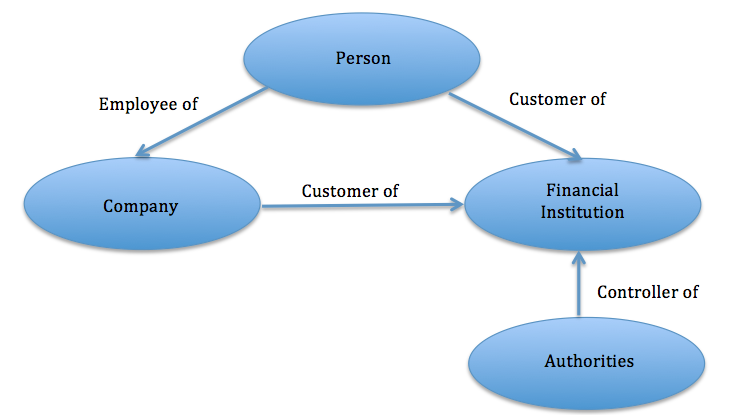
\includegraphics[width=\textwidth]{figures/Customers}
	\caption{Identities in the system}
	\label{fig:Customers}
\end{figure}
\subsection{Private Customers}
Private customers are the individual customers who access Nykredit services on their own. Usually there is a single person accessing the services of the bank. These customers are usually people who get a personal bank account with Nykredit.
\subsection{Corporate Customers}
Corporate customers are either companies who are customers of Nykredit or other financial institutions which provide Nykredit services to their own private customers. Usually there are many people who access Nykredit services on behalf of the corporate customer.
\section{Problem}
We consider the case of a person, who may either be a private customer of Nykredit, or an employee of a company who is corporate customer of Nykredit. In this case, the person may also be responsible for managing the accounts of his employer with Nykredit.
\\
\\Nykredit wants to setup an identity management system so that there is no need for the individual to disclose his personal identity to Nykredit to access the account on behalf of the company.
\\Nykredit, however, also have to comply with relevant legislation (KYC, AML, “Hvidvaskningsloven”),  e.g. in case the authorities (Tax, Police, etc.) find some suspicious transactions. Nykredit needs to provide the identity of the person responsible for these transactions.
This means that it is required that Nykredit, in case of a legal request, is able to identify the individual employee from the institution, who is accessing the account on the corporate customer’s behalf.
\\
\\So the main goal of the system is:
\begin{itemize}
	\item Nykredit should not learn identity of the individual person accessing the services on behalf of corporate customer.
	\item For complying with legislation Nykredit should be able to map real identity of the individual person with the transaction in case its required by the law.
\end{itemize}
The project will perform an initial analysis of a single business process from administrative data management, with respect to identifying the need to bind authenticated identities to actions at the different steps of the process; this analysis will be presented to stakeholders from the specific administrative domain. Based on the initial analysis of the selected business process, the project will develop a full identity model for the chosen business process with anonymisation and pseudonymisation of actors whenever possible. The feasibility of the proposed model will be evaluated through a prototype that implements the model using standard components from identity management infrastructures whenever possible.
\section{Summary}
Companies do not want to disclose the personal identity of their employees to Nykredit, but they still need the ability to access all services online. Managing all identities, while maintaining privacy, is not easy and provides different challenges. We have to design a system, which fulfill the entire privacy requirement and still enables Nykredit to provide its services to its customers and meet the regulatory requirements of the authorities without any problem.
 